%%%%%%%%%%%%%%%%%%%%%%%%%%%%%%%%%%%%%%%%%%%%%%%%%%%%%%%%%%
%%
%% MARK: The Title
%%
%%%%%%%%%%%%%%%%%%%%%%%%%%%%%%%%%%%%%%%%%%%%%%%%%%%%%%%%%%

\chapter*{\S B16. $p$-Forms on Corners}
\setcounter{footnote}{0}

%%%%%%%%%%%%%%%%%%%%%%%%%%%%%%%%%%%%%%%%%%%%%%%%%%%%%%%%%%
%%
%% MARK: Abstract
%%
%%%%%%%%%%%%%%%%%%%%%%%%%%%%%%%%%%%%%%%%%%%%%%%%%%%%%%%%%%

\begin{abstract}
  In this note we shall see that,
  for the subset diffeology,
  differential forms defined on half-spaces or corners of Euclidean spaces
  are the restrictions of differential forms defined on an open neighborhood of the corner in the ambient Euclidean space.
\end{abstract}

%%%%%%%%%%%%%%%%%%%%%%%%%%%%%%%%%%%%%%%%%%%%%%%%%%%%%%%%%%
%%
%% MARK: Introduction
%%
%%%%%%%%%%%%%%%%%%%%%%%%%%%%%%%%%%%%%%%%%%%%%%%%%%%%%%%%%%

Heuristically,
smooth maps from the corner $K^n = \{(x_1,\dots,x_n) \mid x_i \geq 0\}$ into the real line $\RR$ are just defined as restrictions of smooth maps
defined on some open neighborhood of the corner \cite{Cer61} \cite{Dou62} \emph{et al}.
\uline{This heuristic becomes a theorem in diffeology} where $K^n$ is equipped with the subset diffeology.
Indeed,
every map from $K^n$ to $\RR$ which is smooth when composed with any smooth parametrization $P \colon U \to \RR^n$ taking its values in $K^n$
is the restriction of a smooth map defined on some open neighborhood of the corner \cite[\textsection\,4.16]{PIZ13}.

It is always progress when a convention,
based on mathematicians' intuition,
becomes a theorem in a well-defined axiomatic.
Here the axiomatic is the theory of diffeology.
Noting that $\Cinfty(K^n, \RR)$ is just the space of differential $0$-forms $\DForms^0(K^n)$,
it is legitimate to ask about the behavior of differential $k$-forms on $K^n$,
that is,
$\DForms^k(K^n)$ as defined in (op.\,cit \textsection\,6.28).
In this note we prove the following theorem stated in Art. \ref{Differential-Forms-On-Corners}:

\uline{Theorem.} {\itshape Every differential form on the corner $K^n$ is the restriction of a smooth form on an open neighborhood of $K^n$ in $\RR^n$.
Precisely,
the pullback $j^* \colon \DForms^k(\RR^n) \to \DForms^k(K^n)$ is surjective,
where $j$ denotes the inclusion from $K^n$ into $\RR^n$.}

Do we need to remind that a differential $k$-form on a diffeological space $X$ is a mapping $\alpha$ that associates with each plot $P$ in $X$
a smooth $k$-form $\alpha(P)$ on $\Domain(P)$,
such that the smooth compatibility condition $\alpha(F \circ P) = F^*(\alpha(P))$ is satisfied,
where $F$ is any smooth parametrization in $\Domain(P)$.

%%%%%%%%%%%%%%%%%%%%%%%%%%%%%%%%%%%%%%%%%%%%%%%%%%%%%%%%%%
%%
%% MARK: Corners as Diffeologies
%%
%%%%%%%%%%%%%%%%%%%%%%%%%%%%%%%%%%%%%%%%%%%%%%%%%%%%%%%%%%
\section{Smooth structure on corners}

\begin{Article}{Corners as diffeologies.}{}
  We denote by $K^n$ the \emph{corner}
  $$%
    K^n = \{ (x_i)_{i=1}^n \in \RR^n \mid x_i \geq 0,\ i=1,\dots,n\}.
  $$%
  We equip it with the subset diffeology.
  A plot in $K^n$ is just a regular smooth parametrization in $\RR^n$ taking its values in $K^n$.
  
  (A) The corner $K^n$ is the diffeological $n$-fold power of the half-line $K = [0,\infty[ \subset \RR$,
  equipped with the subset diffeology.
  
  (B) The corner $K^n$ is \emph{embedded} in $\RR^n$,
  and closed.
  That is,
  the D-topology of the induction $K^n \subset \RR^n$ coincides with the induced topology%
  \footnote{The standard topology of $\RR^n$ is the D-topology of its standard smooth structure.}
  of $\RR^n$,
  see (op.\,cit \textsection\,2.13).
  
  (C) Let $X_0 = \{0\} \subset X_1 \subset \dots \subset X_n = K^n$ be the natural filtration of $K^n$,
  where the \emph{levels} $X_j$ are defined by
  $$%
    X_j = \{(x_i)_{i=1}^n \in K^n \mid \text{there exist } i_1 < \dots < i_{n-j} \text{ such that } x_{i_\ell} = 0 \}.
  $$%
  Then,
  the \emph{stratum}
  $$%
    S_j = X_j \setminus X_{j-1}
  $$%
  is the subset of points in $\RR^n$ that have exactly $j$ coordinates strictly positive.
  The strata $S_j$ are equipped with the subset diffeology.\footnotemark
  \footnotetext{Recall that,
  by transitivity of the subset diffeology,
  being a subspace of $S_j$ or $K^n$ or $\RR^n$ is identical.}
  
  $$%
    S_j = \bigg\{
    (x_i)_{i=1}^n \in \RR^n \, \bigg| \,
    \begin{array}{l}
    \text{There exist } i_1 < \dots < i_j \text{ such that } x_{i_\ell} > 0, \\
    \text{and } x_m = 0 \text{ for all } m \notin \{i_1,\dots,i_j\}.
    \end{array}
    \bigg\}.
  $$%
  
  Then,
  $S_j$ is D-open in $X_j$ for $j \geq 1$.
  As a subset of $X_j$,
  $S_j$ is the (diffeological) sum of $\binom{n}{j}$ connected components indexed by a string of $j$ ones and $n-j$ zeros.
\end{Article}

\begin{proof}
  For the first item,
  it follows immediately from the definition.
  For the second item:
  for any subset $U \subset K^n$ open in the induced topology,
  there exists (by definition) an open subset $\cO \subset \RR^n$ such that $U = \cO \cap K^n$.
  Then,
  for all plots $P$ in $K^n$,
  $P^{-1}(U) = P^{-1}(\cO)$ is open,
  because plots are continuous.
  On the other hand,
  let $U \subset K^n$ be D-open.
  Then,
  $\Sq^{-1}(U) \subset \RR^n$ is open,
  where $\Sq \colon \RR^n \to K^n$ is the map $\Sq(x_i)_{i=1}^n = (x_i^2)_{i=1}^n$.
  And $\Sq^{-1}(U) \cap K^n$ is open in the induced topology of $\RR^n$.
  Now,
  the map $\Sq$ restricted to $K^n$ is a homeomorphism.
  Hence,
  since $U = \Sq(\Sq^{-1}(U) \cap K^n)$,
  $U$ is open in the induced topology of $\RR^n$.
  Therefore the D-topology of the induction coincides with the induced topology,
  as claimed.
  
  For the third item:
  let $x \in X_j$,
  then the number $\nu$ of vanishing coordinates of $x$ is at least $n-j$,
  i.e., $\nu \geq n-j$.
  Next,
  if $x \in X_j$ and $x \notin X_{j-1}$,
  then $\nu \geq n-j$ and $\nu < n-j+1$,
  thus,
  $\nu = n-j$.
  Therefore,
  $X_j \setminus X_{j-1}$ is the subset of points in $\RR^n$ that have exactly $n-j$ coordinates equal to $0$ and the other $j$ strictly positive.
  
  Consider now a point $x = (x_1,\dots,x_n) \in S_j = X_j \setminus X_{j-1}$.
  Since the $j$ non-zero coordinates of $x$ are strictly positive,
  there exists $\varepsilon > 0$ such that $x_i - \varepsilon > 0$ for each non-zero coordinate of $x$.
  The open $n$-parallelepiped $C_x = ]x_1-\varepsilon,x_1+\varepsilon[ \times \dots \times ]x_n-\varepsilon,x_n+\varepsilon[ \subset \RR^n$ contains $x$,
  and $C_x \cap S_j \subset S_j$.
  Thus,
  $$%
    S_j = \bigcup_{x \in S_j} (C_x \cap S_j).
  $$%
  Now,
  let $P : U \to S_j$ be a plot for the subset diffeology.
  We have,
  $P^{-1}(S_j) = \bigcup_{x \in S_j} P^{-1}(C_x \cap S_j)$,
  but $P^{-1}(C_x \cap S_j) = P^{-1}(C_x)$ since $\Val(P) \subset S_j$.
  Next,
  because $P$ is smooth as a map into $\RR^n$ and $C_x$ is open,
  $P^{-1}(C_x)$ is open and therefore $P^{-1}(S_j)$ is open.
  Hence,
  $S_j$ is D-open in $X_j$.
\end{proof}

\begin{Article}{Smooth maps on corners.}{}
  \label{Smooth-Maps-on-Corners}
  We know that a map $f \colon K^n \to \RR$
  is smooth in the sense of diffeology
  if and only if it is the restriction of a smooth map $F$ defined on some open neighborhood $\cO$ of $K^n$ into $\RR$,
  see (op.\,cit \textsection\,4.16).
  That is,
  $f \in \Cinfty(K^n,\RR)$ if and only if
  $f = F \restriction K^n$ for some $F \in \Cinfty(\cO, \RR)$.
\end{Article}

\begin{Article}{The square function lemma.}{}
  \label{The-Square-Function-Lemma}
  Let $\Sq \colon \RR^n \to K^n$ be the smooth parametrization:
  $$%
    \Sq(x_1,\dots,x_n) = (x_1^2,\dots,x_n^2).
  $$%
  Then $\Sq^* \colon \DForms^k(K^n) \to \DForms^k(\RR^n)$ is injective.
  That is,
  for all $\alpha \in \DForms^k(K^n)$,
  if $\Sq^*(\alpha) = 0$,
  then $\alpha = 0$.
\end{Article}

\begin{proof}
  Note that each component of $S_j$ is isomorphic to $\RR^j$.
  Hence,
  if $\Sq^*(\alpha) = 0$,
  since $\Sq \restriction \Sq^{-1}(S_j)$ is a $2^n$-fold covering over $S_j$,
  we have $\alpha \restriction S_j = 0$.
  That is,
  for all plots $Q$ in $S_j$,
  $\alpha(Q)=0$.
  
  Now,
  for some $j \geq 1$,
  let $P_j \colon U_j \to X_j$ be a plot.
  In view of what precedes,
  the subset $\cO_j = P_j^{-1}(S_j)$ is open,
  and $\alpha(P_j \restriction \cO_j) = \alpha(P_j) \restriction \cO_j = 0$.
  By continuity,
  $\alpha(P_j) \restriction \overline{\cO}_j = 0$,
  where $\overline{\cO}_j$ is the closure of $\cO_j$.
  Let then $U_{j-1} = U_j \setminus \overline{\cO}_j$ and $P_{j-1} = P_j \restriction U_{j-1}$.
  Then,
  $U_{j-1}$ is open and $P_{j-1} \colon U_{j-1} \to X_{j-1}$ is a plot.
  
  This construction gives a descending recursion,
  starting with any plot $P \colon U \to K^n$,
  by initializing $P_n = P$,
  $U_n = U$ and $X_n = K^n$.
  One has $P_j = P \restriction U_j$,
  $U_{j-1} \subset U_j$,
  the recursion ends with a plot $P_0$ with values in $X_0 = \{0\}$,
  and $\alpha(P_0) = 0$ since $P_0$ is constant.
  
  Therefore $\alpha = 0$.
\end{proof}

\begin{Article}{Differential forms on corners.}{}
  \label{Differential-Forms-On-Corners}
  The previous article (art. \ref{Smooth-Maps-on-Corners}) deals with smooth real functions on corners,
  that is,
  $\DForms^0(K^n)$.
  It is a particular case of the more general theorem:
  
  \textsc{Theorem.} \itshape Any differential $k$-form on the corner $K^n$,
  equipped with the subset diffeology of $\RR^n$,
  is the restriction of a smooth differential $k$-form defined on some open neighborhood of the corner.
  Precisely,
  the pullback $j^* \colon \DForms^k(\RR^n) \to \DForms^k(K^n)$ is surjective,
  where $j$ denotes the inclusion from $K^n$ into $\RR^n$.
\end{Article}

\begin{proof}
  Let $\omega \in \DForms^k(K^n)$ and $\mathring K^n = \{ (x_i)_{i=1}^n \mid x_i > 0,\ i=1,\dots,n \}$.
  One has
  $$%
    \omega \restriction \mathring K^n = \sum_{i_1<\dots<i_k} a_{i_1 \dots i_k}(x_1, \dots, x_n)\ dx_{i_1} \wedge \dots \wedge dx_{i_k},
  $$%
  with $i_j = 1,\dots,n$ and $a_{i_1 \dots i_k} \in \Cinfty(\mathring K^n,\RR)$.
  Recall that $\Sq \colon (x_i)_{i=1}^n \mapsto (x_i^2)_{i=1}^n$,
  then
  $$%
    \Sq^*(\omega) = \sum_{i_1<\dots<i_k} A_{i_1 \dots i_k}(x_1,\dots, x_n)\ dx_{i_1} \wedge \dots \wedge dx_{i_k},
  $$%
  where $A_{i_1 \dots i_k} \in \Cinfty(\RR^n,\RR)$.
  Let $\varepsilon_j : (\dots, x_j,\dots) \mapsto (\dots, -x_j,\dots)$.
  Then $\Sq \circ \varepsilon_j = \Sq$ and $(\Sq \circ \varepsilon_j)^*(\omega) = \varepsilon_j^*(\Sq^*(\omega))$,
  that is,
  $\Sq^*(\omega) = \varepsilon_j^*(\Sq^*(\omega))$.
  Hence,
  \begin{multline*}
    \varepsilon_j^*(\Sq^*(\omega)) = \sum_{\substack{i_1<\dots<i_k \\ i_\ell \neq j}} A_{i_1 \dots i_k}(x_1,\dots, -x_j,\dots, x_n)\ dx_{i_1} \wedge \dots \wedge dx_{i_k} \\
    - \sum_{\substack{i_1 < \dots < j < \dots < i_k}} A_{i_1\dots j \dots i_k}(x_1,\dots, -x_j,\dots, x_n)\ dx_{i_1} \wedge \dots \wedge dx_j \wedge \dots \wedge dx_{i_k}.
  \end{multline*}
  Then,
  \begin{eqnarray*}
    A_{\substack{i_1 \dots i_k \\ i_\ell \neq j}}(x_1,\dots, -x_j,\dots, x_n) & = & A_{i_1 \dots i_k}(x_1,\dots, x_j,\dots, x_n), \\
    A_{i_1 \dots j \dots i_k}(x_1,\dots, -x_j,\dots, x_n) & = & - A_{i_1\dots j \dots i_k}(x_1,\dots, x_j,\dots, x_n).
  \end{eqnarray*}
  Hence,
  $$%
    A_{i_1 \dots j \dots i_k}(x_1,\dots, x_j=0,\dots, x_n) = 0.
  $$%
  Thus,
  $$%
    A_{i_1\dots j \dots i_k}(x_1,\dots, x_j,\dots, x_n) = 2 x_j \underline{A}_{i_1\dots j \dots i_k}(x_1,\dots, x_j,\dots, x_n),
  $$%
  with $\underline{A}_{i_1\dots j \dots i_k} \in \Cinfty(\RR^n,\RR)$.
  Therefore,
  there exist smooth functions $\hat A_{i_1\dots i_k}$ defined on $\RR^n$ such that
  $$%
    A_{i_1 \dots i_k}(x_1,\dots, x_n) = 2^k x_{i_1}\dots x_{i_k} \hat A_{i_1\dots i_k}(x_1,\dots, x_n).
  $$%
  Now,
  $$%
    \Sq^*(\omega\restriction \mathring K^n) = \Sq^*(\omega) \restriction \{x_i \neq 0\}
  $$%
  implies
  \begin{align*}
     \sum_{i_1<\dots<i_k} 2^k x_{i_1}\dots x_{i_k} a_{i_1 \dots i_k}(x_1^2,\dots, x_n^2)\ dx_{i_1} \wedge \dots \wedge dx_{i_k} \\
     = \sum_{i_1<\dots<i_k} 2^k x_{i_1}\dots x_{i_k} \hat A_{i_1 \dots i_k}(x_1,\dots, x_n) \ dx_{i_1} \wedge \dots \wedge dx_{i_k}.
  \end{align*}
  Hence,
  $$%
    \hat A_{i_1 \dots i_k}(x_1,\dots, x_n) = a_{i_1 \dots i_k}(x_1^2,\dots, x_n^2) \quad \text{for } x_i \neq 0,\ i = 1,\dots,n.
  $$%
  Thus $(x_1,\dots, x_n) \mapsto \hat A_{i_1 \dots i_k}(x_1,\dots, x_n)$,
  which belongs to $\Cinfty(\RR^n,\RR)$,
  is even in each variable.
  Therefore,
  according to Schwartz's theorem \cite{Sch75},%
  \footnote{Which is a generalization of the famous Whitney theorem \cite{Whi43}.}
  there exists
  $$%
    \underline{a}_{i_1 \dots i_k} \in \Cinfty(\RR^n,\RR)
  $$%
  such that
  $$%
    \hat A_{i_1 \dots i_k}(x_1,\dots, x_n) = \underline{a}_{i_1 \dots i_k}(x_1^2,\dots, x_n^2).
  $$%
  One deduces:
  $$%
    \underline{a}_{i_1 \dots i_k}(x_1,\dots, x_n) = a_{i_1 \dots i_k}(x_1,\dots, x_n) \quad \text{for all } (x_1,\dots, x_n) \in \mathring{K}^n.
  $$%
  Then,
  defining the $k$-form $\underline\omega$ on $\RR^n$ by
  $$%
    \underline\omega = \sum_{i_1<\dots<i_k} \underline{a}_{i_1 \dots i_k}(x_1, \dots, x_n)\ dx_{i_1} \wedge \dots \wedge dx_{i_k},
  $$%
  one already has
  $$%
    \underline\omega \restriction \mathring K^n = \omega \restriction \mathring K^n.
  $$%
  Let us show that $\underline\omega \restriction K^n = \omega$.
  That is,
  let us check that for all plots $P \colon U \to \RR^n$,
  $P^*(\underline\omega) = \omega(P)$.
  Actually,
  one has
  $$%
    \Sq^*(\omega) = \Sq^*(\underline\omega \restriction K^n).
  $$%
  Indeed:
  \begin{align*}
    \Sq^*(\omega) & = \sum_{i_1\dots i_k} A_{i_1\dots i_k}(x_1,\dots,x_n)\ dx_{i_1}\wedge\dots\wedge dx_{i_k} \\
    & = \sum_{i_1\dots i_k} 2^k x_{i_1} \dots x_{i_k} \hat A_{i_1\dots i_k}(x_1,\dots,x_n)\ dx_{i_1}\wedge\dots\wedge dx_{i_k} \\
    & =  \sum_{i_1\dots i_k} 2^k x_{i_1} \dots x_{i_k} \underline{a}_{i_1\dots i_k}(x_1^2,\dots,x_n^2)\ dx_{i_1}\wedge\dots\wedge dx_{i_k}.
  \end{align*}
  And,
  on the other hand:
  \begin{eqnarray*}
    \Sq^*(\underline\omega\restriction K^n) = \sum_{i_1\dots i_k} 2^k x_{i_1} \dots x_{i_k} \underline{a}_{i_1\dots i_k}(x_1^2,\dots,x_n^2)\ dx_{i_1}\wedge\dots\wedge dx_{i_k}.
  \end{eqnarray*}
  Thus,
  $\Sq^*(\omega - \underline\omega \restriction K^n) = 0$.
  Therefore,
  according to the previous lemma (art. \ref{The-Square-Function-Lemma}),
  $\omega - \underline\omega \restriction K^n = 0$.
  And indeed,
  $\omega$ is the restriction of the smooth $k$-form $\underline\omega$ to $K^n$.
\end{proof}

%%%%%%%%%%%%%%%%%%%%%%%%%%%%%%%%%%%%%%%%%%%%%%%%%%%%%%%%%%
%%
%% MARK: Corners as Diffeologies
%%
%%%%%%%%%%%%%%%%%%%%%%%%%%%%%%%%%%%%%%%%%%%%%%%%%%%%%%%%%%
\section{Application}

\begin{Article}{An example of application.}{}
  \label{An-Example-Of-Application}
  Among the possible applications of the theorems above (art. \ref{The-Square-Function-Lemma} and \ref{Differential-Forms-On-Corners}),
  there is already one worthy of mention.
  It concerns the description of closed $2$-forms
  invariant under the action of a Lie group.
  As was shown in particular in the classification of $\SO(3)$-symplectic manifolds \cite{Igl84,Igl91},
  any closed $2$-form $\omega$ on a manifold $M$
  invariant under a compact group%
  \footnote{A diffeological generalization to non-compact groups may be possible.}
  $G$
  is characterized by its \emph{moment map} $\mu \colon M \to \cG^*$ (assuming the action is Hamiltonian),
  together with a closed $2$-form $\varepsilon \in Z^2(M/G)$.
  Let us be precise:
  the space of closed $2$-forms $Z^2(M)$ is a vector space,
  and the space of $G$-equivariant maps from $M$ to $\cG^*$ is also a vector space.
  Then,
  the map associating its moment map%
  \footnote{The manifold $M$ is assumed to be connected.
  To ensure uniqueness of the moment maps we fix their value to $0$ at some base point $m_0 \in M$, for example.}
  $\mu$ to each invariant closed $2$-form $\omega$ is linear.
  What we claim is that the kernel of this map is exactly $Z^2(M/G)$,
  where $M/G$ is equipped with the quotient diffeology.
  
  Now,
  while an equivariant map is easy to conceive,
  a differential form on the space of orbits is more problematic,
  since this space is generally not a manifold.
  This is where the above theorem can help,
  because it happens that $M/G$ is not far from being a manifold with boundary or corners,
  as the following example shows.
  
  Consider the simple case of $M = \RR^{2n}$ equipped with the standard symplectic form $\omega = \sum_{i=1}^n dq_i \wedge dp_i$.
  This form is invariant under the natural action of the group $\SO(2,\RR)^n$,
  each factor acting on its respective copy of $\RR^2$.
  The (diffeological) quotient space $\cQ^n = \RR^{2n}/\SO(2,\RR)^n$ is the $n$-fold power of $\cQ = \RR^2/\SO(2,\RR)$.
  Let $X = (X_i)_{i=1}^n$ with $X_i = (q_i,p_i)$.
  There is a natural smooth bijection $j_{2n} \colon \cQ^n \to K^n$,
  given by $j_{2n} \colon \Class(X) \mapsto (\|X_i\|^2)_{i=1}^n$.
  It turns out that this smooth bijection%
  \footnote{Which is not a diffeomorphism \cite{PIZ07}.}
  induces,
  by pullback,
  an injection $j_{2n}^*$ from $\DForms^k(K^n)$ into $\DForms^k(\cQ^n)$.
  Thus,
  thanks to Art.~\ref{Differential-Forms-On-Corners},
  for each $k$-form $\varepsilon$ on the quotient $\cQ^n$ there exists a $k$-form $\underline \varepsilon$ on $\RR^n$
  such that $\varepsilon = j_{2n}^*(\underline\varepsilon)$.
  And the $2$-form $\omega$ is characterized by $\mu$ and $\underline \varepsilon \restriction K^n$,
  with $\underline \varepsilon \in \DForms^k(\RR^n)$.
\end{Article}

\begin{proof}
  Let us prove that $j_{2n}^*$ is injective.
  Let $x = (x_i)_{i=1}^n \in \RR^n$ and $\iota_n \colon x \mapsto (x_i,0)_{i=1}^n$ from $\RR^n$ into $\RR^{2n}$.
  Let $j_n \colon \RR^n/\{\pm1\}^n \to K^n$ be defined by $j_n \colon \Class(x) \mapsto \Sq(x) = (x_i^2)_{i=1}^n$.
  Then,
  $j_n = j_{2n} \circ \underline{\iota}$,
  where $\underline{\iota}$ is the projection of $\iota$,
  from $\RR^n/\{\pm1\}^n$ to $\cQ^n$.
  $$%
    \begin{tikzcd}[column sep=large, row sep=large, every label/.append style = {font = \small}]
    \RR^n \arrow[d, swap, "\Class"] \arrow[r, "\iota"] &  \RR^{2n} \arrow[d, "\Class"] &  \\
    \RR^n/\{\pm1\}^n \arrow[r, swap, "\underline \iota"] & \cQ^n = \RR^{2n}/\SO(2,\RR)^n \arrow[r, swap, "j_{2n}"] & K^n = [0,\infty[^{\,n}
    \end{tikzcd}
  $$%
  But $\Sq = j_n \circ \Class$ and we know that $\Sq^* = \Class^* \circ j_n^* \colon \DForms^k(K^n) \to \DForms^k(\RR^n)$ is injective by Art~\ref{The-Square-Function-Lemma},
  thus $j_n^* \colon \DForms^k(K^n) \to \DForms^k(\RR^n/\{\pm1\}^n)$ is injective.
  On the other hand,
  $j_n = j_{2n} \circ \underline\iota$,
  hence $j_n^* = \underline\iota^* \circ j_{2n}^*$.
  Since $j_n^*$ is injective,
  $j_{2n}^*$ is necessarily injective as well.
\end{proof}

\vfill
\centerline{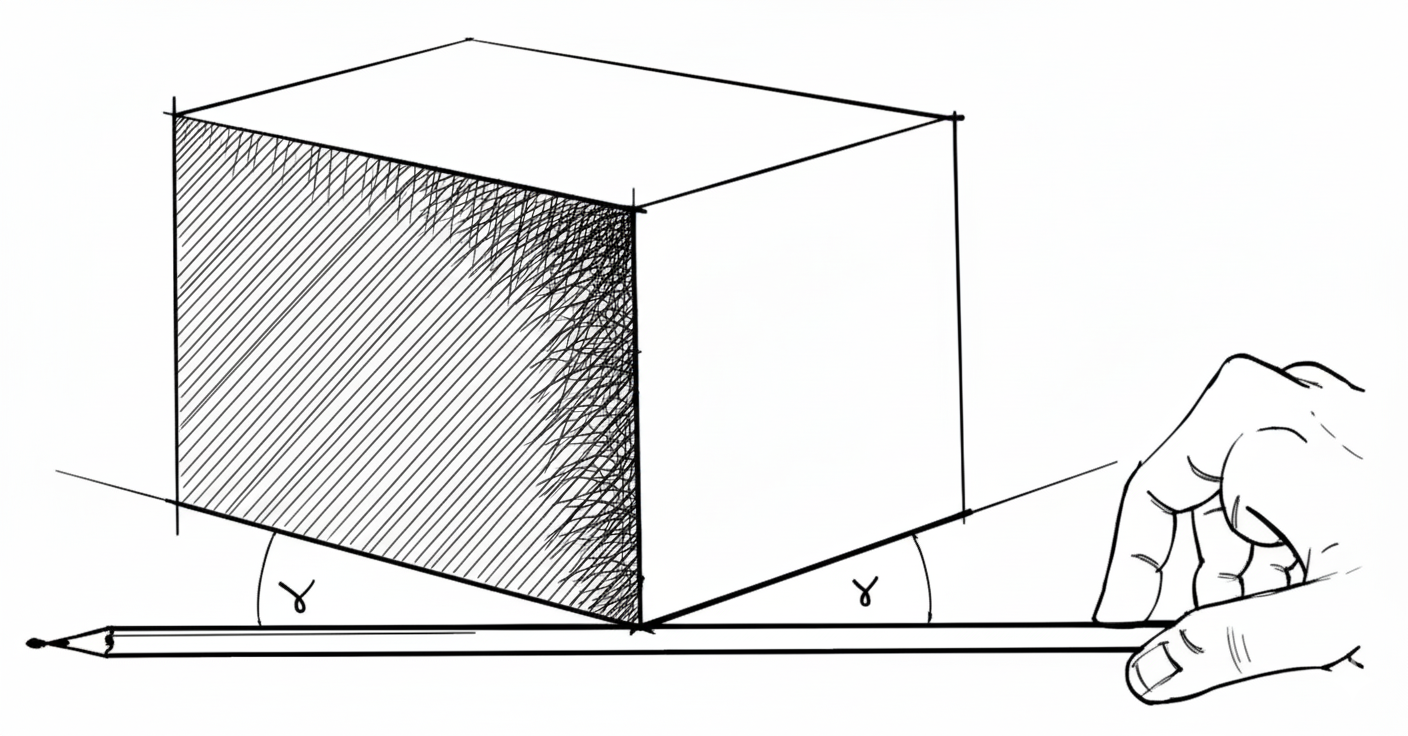
\includegraphics[width=.72\textwidth]{Figures/cube.png}}
\vfill
